\documentclass[12pt]{article}

\usepackage{amsmath}
\usepackage{amssymb}
\usepackage{enumitem}
\usepackage{geometry}
\geometry{margin=1in}

\usepackage{tikz}
\usetikzlibrary{
    arrows.meta,
    calc,
    angles,
    quotes,
    decorations.pathmorphing
}
\usepackage[american]{circuitikz}



\setlist[enumerate,1]{label=\arabic*.}

\begin{document}

\begin{center}
\Large \textbf{ULTRA-HARD PHYSICS PAPER — SINGLE CORRECT}
\end{center}

\begin{enumerate}

%=========================================================

%=========================================================

\item
A uniform solid cylinder of mass $M$ and radius $R$ rolls without slipping on a rough horizontal surface while a horizontal force $F$ is applied at its centre. A small block of mass $m$ is gently placed at the topmost point of the cylinder and remains in contact due to friction between block and cylinder. Assume coefficient of friction between the block and cylinder is $\mu$, while the ground is sufficiently rough to prevent slipping of the cylinder. 

Assume that the motion is analysed in the small-speed regime so that the centripetal reduction of normal reaction at the topmost point may be neglected. Determine the maximum value of $F$ for which the block does not slip relative to the cylinder.

\begin{center}
\begin{tikzpicture}[scale=1]

% Ground
\draw (-4,-1.8)--(4,-1.8);

% Cylinder
\draw (0,0) circle (1.5);

% Block
\draw (-0.4,1.5)--(0.4,1.5)--(0.4,2.1)--(-0.4,2.1)--cycle;
\node at (0,1.8) {$m$};

% Center
\node at (0,0) {$M$};

% Force
\draw[->, thick] (0,0)--(2,0);
\node[right] at (2,0) {$F$};

% Rolling arrow
\draw[->, thick] (1.1,0.8) arc (40:300:1);

\end{tikzpicture}
\end{center}

\begin{enumerate}[label=\Alph*)]
\item $\dfrac{3}{4}M\mu g$
\item $\dfrac{3}{2}M\mu g$
\item $\dfrac{1}{2}M\mu g$
\item $\dfrac{2}{3}M\mu g$
\end{enumerate}
%=========================================================

\item
A small bead of mass $m$ is constrained to move without friction on a rigid circular ring of radius $R$. The ring rotates with constant angular velocity $\omega$ about its vertical diameter in a uniform gravitational field $g$. Using stability analysis of equilibrium positions in the rotating frame, determine the critical angular speed at which the lowest equilibrium position loses stability and bifurcation of equilibrium occurs.


\begin{center}
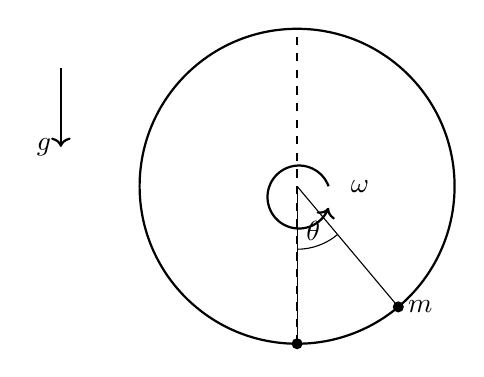
\begin{tikzpicture}[scale=1]

\def\R{2}
\def\ang{40}

% Ring
\draw[thick] (0,0) circle (\R);

% Vertical diameter (axis)
\draw[dashed, thick] (0,-\R)--(0,\R);



% Angular velocity arrow about vertical axis
\draw[->, thick] (0.4,0) arc (20:340:0.4);
\node at (.8,0) {$\omega$};

% Gravity arrow
\draw[->, thick] (-3,1.5)--(-3,0.5);
\node[left] at (-3,0.5) {$g$};

% Lowest point
\fill (0,-\R) circle (2pt);

% Bead
\coordinate (bead) at ({\R*sin(\ang)},{-\R*cos(\ang)});
\fill (bead) circle (2pt);
\node[right] at (bead) {$m$};

% Radius lines
\draw (0,0)--(bead);
\draw (0,0)--(0,-\R);

% Theta arc
\draw (0,-0.8) arc (-90:{-90+\ang}:0.8);
\node at ({0.6*sin(\ang/2)},{-0.6*cos(\ang/2)}) {$\theta$};

\end{tikzpicture}
\end{center}

\begin{enumerate}[label=\Alph*)]
\item $\sqrt{\dfrac{g}{R}}$
\item $\sqrt{\dfrac{2g}{R}}$
\item $\sqrt{\dfrac{g}{2R}}$
\item $\sqrt{\dfrac{3g}{R}}$
\end{enumerate}

%=========================================================

%=========================================================

\item
A square conducting loop of side $a$ and resistance $R$ moves with constant velocity $v$ towards a region of uniform magnetic field $B$ directed perpendicular to the plane of the loop. The magnetic field occupies a semi-infinite region with sharp boundary. Determine the maximum induced current during the entry phase considering the time variation of magnetic flux and the transient change in effective length inside the field.

\begin{center}
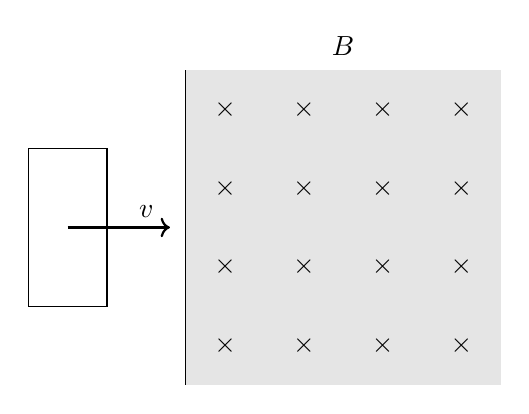
\begin{tikzpicture}[scale=1]

% Boundary of magnetic field
\draw (0,0)--(0,4);

% Field region shading
\fill[gray!20] (0,0)--(4,0)--(4,4)--(0,4)--cycle;

% Magnetic field crosses
\foreach \x in {0.5,1.5,2.5,3.5}
  \foreach \y in {0.5,1.5,2.5,3.5}
    \node at (\x,\y) {$\times$};

% Loop
\draw (-2,1)--(-1,1)--(-1,3)--(-2,3)--cycle;

% Velocity arrow (CORRECTED)
\draw[->, thick] (-1.5,2)--(-0.2,2);
\node[above] at (-0.5,2) {$v$};

% Label B
\node at (2,4.3) {$B$};

\end{tikzpicture}
\end{center}

\begin{enumerate}[label=\Alph*)]
\item $\dfrac{Bav}{R}$
\item $\dfrac{Ba^2v}{R}$
\item $\dfrac{Bv}{R}$
\item $\dfrac{Ba^2}{R}$
\end{enumerate}

%=========================================================

\item
An ideal gas is confined inside a vertical cylinder fitted with a frictionless piston of mass $M$ attached to a vertical spring of spring constant $k$. The system is initially in equilibrium under gravity $g$. The entire arrangement is placed inside an elevator accelerating upward with constant acceleration $a$. Determine the fractional change in angular frequency of small oscillations of the piston-gas system about the new equilibrium position, accounting for effective gravity and thermodynamic restoring force.

\begin{enumerate}[label=\Alph*)]
\item $\dfrac{a}{2g}$
\item $\dfrac{a}{g}$
\item $\dfrac{a}{g+a}$
\item independent of $a$
\end{enumerate}

%=========================================================

\item
A particle of mass $m$ and charge $q$ moves in a region where magnetic field varies linearly with vertical coordinate as $B(y)=B_0+\alpha y$. The particle is projected horizontally with speed $v$ at $y=0$. Assuming motion remains approximately circular locally, determine the radius of curvature as a function of height $y$ using Lorentz force balance and local field approximation.

\begin{enumerate}[label=\Alph*)]
\item $\dfrac{mv}{q(B_0+\alpha y)}$
\item $\dfrac{mv}{qB_0}$
\item $\dfrac{mv}{q\alpha y}$
\item $\dfrac{mv(B_0+\alpha y)}{q}$
\end{enumerate}

%=========================================================

%=========================================================

\item
Two identical blocks each of mass $m$ are connected by a light spring of spring constant $k$ and placed on a smooth horizontal surface. One block carries charge $q$ while the other is neutral. A uniform electric field $E$ is suddenly switched on parallel to the line joining the blocks when the spring is initially relaxed. Determine the maximum compression of the spring during subsequent motion using centre of mass and relative motion analysis.

\begin{enumerate}[label=\Alph*)]
\item $\dfrac{qE}{2k}$
\item $\dfrac{qE}{k}$
\item $\dfrac{qE}{4k}$
\item $\dfrac{2qE}{k}$
\end{enumerate}



%=========================================================

\item
A satellite revolves in a circular orbit of radius $R$ around Earth. Due to slow isotropic radiation, Earth’s mass decreases at a constant rate while no external torque acts on the satellite. Assuming orbital angular momentum remains conserved at each instant, determine how the orbital radius changes with time and identify the proportional dependence of $\frac{dR}{dt}$ on $R$.

\begin{enumerate}[label=\Alph*)]
\item $\dfrac{dR}{dt}\propto R$
\item $\dfrac{dR}{dt}\propto \dfrac{1}{R}$
\item $\dfrac{dR}{dt}\propto \dfrac{1}{R^2}$
\item constant
\end{enumerate}

%=========================================================

\item
A particle oscillates in a one-dimensional potential given by  
\[
U(x)=\alpha x^4+\frac{1}{2}kx^2.
\]
Assuming small anharmonicity and oscillation amplitude $A$, determine the leading order correction to oscillation frequency using energy method or perturbative approach. Identify how the correction depends on amplitude and anharmonic coefficient.

\begin{enumerate}[label=\Alph*)]
\item $\alpha A^2$
\item $\alpha A^4$
\item $\dfrac{\alpha}{A^2}$
\item constant
\end{enumerate}

%=========================================================

\item
A charged particle is projected into mutually perpendicular uniform electric and magnetic fields such that electric field magnitude slightly exceeds the velocity selector condition. Analyse the motion using drift velocity concept and determine the qualitative nature of trajectory observed in laboratory frame.

\begin{enumerate}[label=\Alph*)]
\item cycloidal
\item straight line
\item spiral
\item uniform circular
\end{enumerate}

%=========================================================

%=========================================================

\item
A light rigid rod of length $L$ carries equal masses $m$ at its ends and is constrained to rotate in a vertical plane about its midpoint. The system is driven so that angular speed increases slowly. Determine the critical angular speed at which the vertical equilibrium configuration loses stability.

\begin{enumerate}[label=\Alph*)]
\item $\sqrt{\dfrac{g}{L}}$
\item $\sqrt{\dfrac{2g}{L}}$
\item $\sqrt{\dfrac{4g}{L}}$
\item $\sqrt{\dfrac{g}{2L}}$
\end{enumerate}

%=========================================================

\item
A parallel plate capacitor partially filled with dielectric is connected to a constant voltage battery. The dielectric slab is slowly withdrawn while maintaining electrical connection. Considering change in stored energy and work done by battery, determine the work done by the external agent during the process.

\begin{enumerate}[label=\Alph*)]
\item increase in electrostatic energy
\item decrease in electrostatic energy
\item zero
\item half increase
\end{enumerate}

%=========================================================

\item
A particle is released from rest at the top of a smooth vertical circular track of radius $R$ and just manages to complete the loop without losing contact. Using energy conservation and normal reaction condition at the topmost point, determine the minimum speed required at the lowest point.

\begin{enumerate}[label=\Alph*)]
\item $\sqrt{5gR}$
\item $\sqrt{4gR}$
\item $\sqrt{3gR}$
\item $\sqrt{2gR}$
\end{enumerate}

%=========================================================

\item
A conducting rod of length $L$ moves with constant velocity perpendicular to both its length and a uniform magnetic field. Taking into account motional emf and charge separation until electrostatic equilibrium is established, determine the potential difference between its ends.

\begin{enumerate}[label=\Alph*)]
\item $BLv$
\item $Bv$
\item $Lv$
\item zero
\end{enumerate}

%=========================================================

\item
Consider an electron in the ground state of Bohr hydrogen atom. If Planck’s constant were hypothetically doubled while all other constants remain unchanged, determine how the radius of the orbit changes according to Bohr quantization condition.

\begin{enumerate}[label=\Alph*)]
\item $4r$
\item $2r$
\item $r$
\item $\dfrac{r}{2}$
\end{enumerate}

%=========================================================

\item
A damped harmonic oscillator with damping constant $b$ executes motion described by  
\[
x=Ae^{-\beta t}\cos\omega t.
\]
Determine the ratio of total mechanical energies at two successive maxima of displacement by analysing exponential decay of amplitude and relation between energy and amplitude.

\begin{enumerate}[label=\Alph*)]
\item $e^{-2\pi\beta/\omega}$
\item $e^{-4\pi\beta/\omega}$
\item $e^{-2\beta/\omega}$
\item $e^{-\beta/\omega}$
\end{enumerate}

%=========================================================

\end{enumerate}

\end{document}